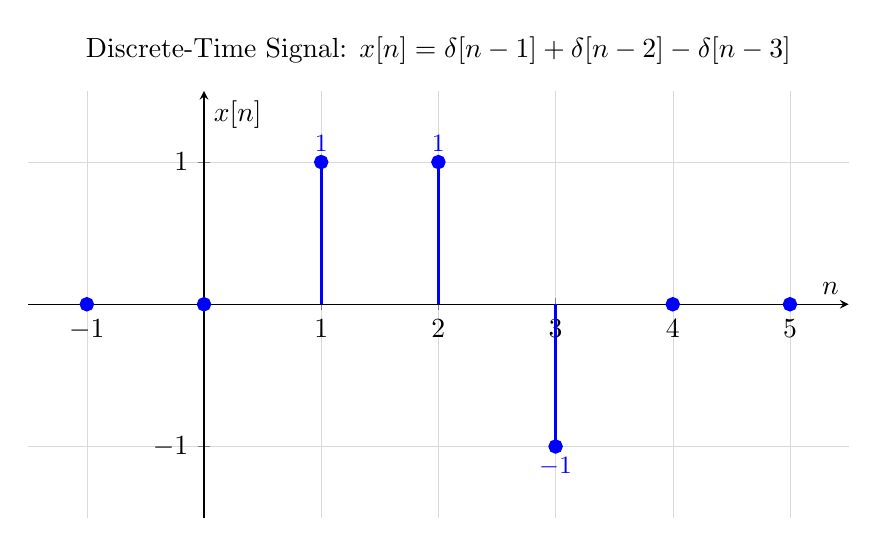
\begin{tikzpicture}
	% Define a style for our stem plots
	\pgfplotsset{
		impulse/.style={
			ycomb,          % Use the 'ycomb' style for stems
			blue,           % Ensure stems and markers are blue
			very thick,     % Thickness of the stems
			mark=*,         % Marker style at the tip of the stem
			mark size=2pt,  % Size of the marker
			draw=blue,      % Ensure the drawing color is blue
			fill=blue,      % Ensure the marker fill is blue
		}
	}
	
	\begin{axis}[
		width=12cm,
		height=7cm,
		title={Discrete-Time Signal: $x[n] = \delta[n-1] + \delta[n-2] - \delta[n-3]$},
		xlabel={$n$},
		ylabel={$x[n]$},
		axis lines=middle,
		xmin=-1.5, xmax=5.5,
		ymin=-1.5, ymax=1.5,
		xtick={-1,0,...,5},
		ytick={-1, 1},
		grid=major,
		grid style={line width=.1pt, draw=gray!30},
		]
		
		% Plot the positive impulses with labels above
		\addplot[
		impulse,
		nodes near coords, % Add value labels
		every node near coord/.style={anchor=south, font=\small}, % Labels above
		] coordinates {
			(1, 1)
			(2, 1)
		};
		
		% Plot the negative impulses with labels below
		\addplot[
		impulse,
		nodes near coords, % Add value labels
		every node near coord/.style={anchor=north, font=\small}, % Labels below
		] coordinates {
			(3, -1)
		};
		
		% Plot the zero-value points (no labels needed)
		\addplot[impulse] coordinates {
			(-1, 0)
			(0, 0)
			(4, 0)
			(5, 0)
		};
		
	\end{axis}
\end{tikzpicture}